% ---------------------------------------------------------------------
% Report skeleton — Day 1 stub. Only §Methodology and Appendix A are
% drafted here (STEPS.md §1.7); other sections are placeholders filled
% on Days 2–4 (STEPS.md §2.2, §3.4, §4.2).
%
% Build:   latexmk -pdf main.tex      (from report/)
% ---------------------------------------------------------------------
\documentclass[11pt,a4paper]{article}

\usepackage[utf8]{inputenc}
\usepackage[T1]{fontenc}
\usepackage[margin=2.5cm]{geometry}
\usepackage{booktabs}
\usepackage{listings}
\usepackage{xcolor}
\usepackage{tikz}
\usetikzlibrary{arrows.meta, positioning}
\usepackage{hyperref}

\lstset{
  basicstyle=\ttfamily\small,
  breaklines=true,
  frame=single,
  framerule=0pt,
  backgroundcolor=\color{black!3},
  showstringspaces=false,
  keepspaces=true,
  columns=flexible,
}

\title{Controlled Comparative Study of LLM Planning\\
       \large Unifying Merola~et~al.\ (Project~A) and
       D'Ascenzo~\&~Gentili (Project~B)}
\author{Usama Shabbir Satti \and Muhammad Fahim Asim \and Hassan Ahmed Mujtaba}
\date{April 2026 --- Day~1 draft}

\begin{document}
\maketitle

\begin{abstract}
% Fill on Day 3 once Results are in.
\noindent\textit{Abstract --- to be written on Day~3 once the 18-cell
results matrix is populated.}
\end{abstract}

% \input{context}           % Day 4
% \input{experimental_design}   % Day 4
% ---------------------------------------------------------------------
% Methodology — first draft (STEPS.md §1.7).
% Self-contained section; input from main.tex via % ---------------------------------------------------------------------
% Methodology — first draft (STEPS.md §1.7).
% Self-contained section; input from main.tex via % ---------------------------------------------------------------------
% Methodology — first draft (STEPS.md §1.7).
% Self-contained section; input from main.tex via \input{methodology}.
% Appendix with the 6 reference prompts lives in appendix_prompts.tex.
% ---------------------------------------------------------------------

\section{Methodology}
\label{sec:methodology}

This section describes the unified pipeline used to run
$3\ \text{models} \times 3\ \text{domains} \times 2\ \text{prompting conditions} = 18$
experimental cells, and the mechanical steps we took to keep every
cell comparable. The key design commitment is that the only thing that
varies between two cells is the axis being studied --- the model, the
domain, or the prompting condition. Everything else (prompt shell,
generation configuration, iteration policy, validator) is controlled
by a single source of truth and verified on disk before and after the
SLURM runs.

\subsection{Pipeline overview}
\label{sec:methodology:pipeline}

Figure~\ref{fig:pipeline} shows the end-to-end flow. A parametric
SLURM entry point
(\texttt{scripts/slurm/run.sh}) accepts three environment variables
--- \texttt{MODEL}, \texttt{DOMAIN}, \texttt{CONDITION} --- and is submitted
18 times by \texttt{scripts/slurm/submit\_all.sh}. Each job loads one
model once, iterates over the 20 instances of the assigned domain,
and for every instance runs a prompt $\rightarrow$ generate $\rightarrow$
validate loop with up to 4 iterations under a stop-on-success policy
(Section~\ref{sec:methodology:iteration}). Per-iteration rows are
appended to \texttt{run\_metrics.csv}; the final plan is written to
\texttt{instance-XX\_plan.txt} with a metadata block that records
\texttt{first\_valid\_iter}.

\begin{figure}[t]
\centering
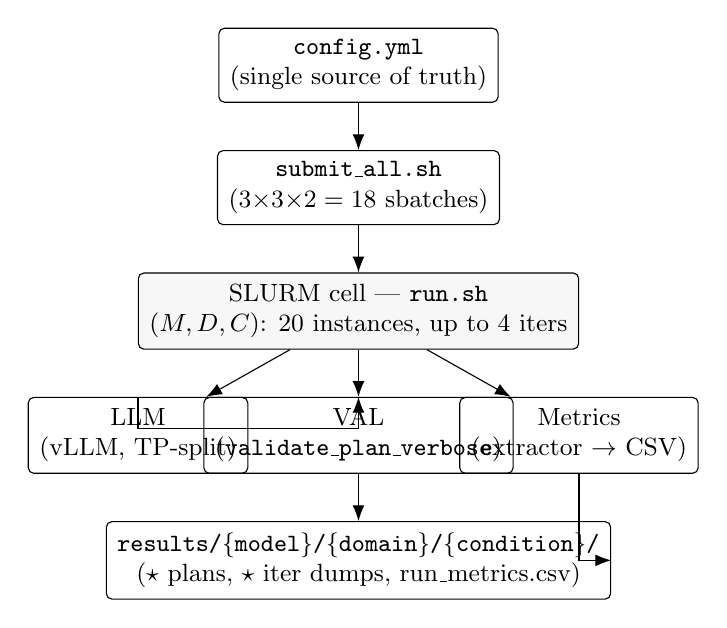
\begin{tikzpicture}[
    node distance=6mm and 10mm,
    box/.style={draw, rounded corners=2pt, align=center,
                minimum height=8mm, inner sep=4pt, font=\small},
    cell/.style={draw, rounded corners=2pt, align=center,
                 fill=black!3, minimum height=8mm, inner sep=4pt,
                 font=\small},
    arr/.style={-{Latex[length=2mm]}}
]
\node[box]                                      (cfg)   {\texttt{config.yml}\\(single source of truth)};
\node[box, below=of cfg]                        (sub)   {\texttt{submit\_all.sh}\\($3{\times}3{\times}2 = 18$ sbatches)};
\node[cell, below=of sub]                       (cell)  {SLURM cell --- \texttt{run.sh}\\$(M, D, C)$: 20 instances, up to 4 iters};
\node[box, below=of cell, xshift=-28mm]         (llm)   {LLM\\(vLLM, TP-split)};
\node[box, below=of cell]                       (val)   {VAL\\(\texttt{validate\_plan\_verbose})};
\node[box, below=of cell, xshift=28mm]          (met)   {Metrics\\(extractor $\to$ CSV)};
\node[box, below=of val]                        (out)   {\texttt{results/\{model\}/\{domain\}/\{condition\}/}\\($\star$ plans, $\star$ iter dumps, run\_metrics.csv)};

\draw[arr] (cfg)  -- (sub);
\draw[arr] (sub)  -- (cell);
\draw[arr] (cell) -- (llm);
\draw[arr] (cell) -- (val);
\draw[arr] (cell) -- (met);
\draw[arr] (llm)  |- ([yshift=-4mm]val.north) -- (val);
\draw[arr] (val)  -- (out);
\draw[arr] (met)  |- (out);
\end{tikzpicture}
\caption{Pipeline overview. \texttt{config.yml} is loaded once per job
and echoed to stdout at job start (Section~\ref{sec:methodology:genconfig}),
giving a post-hoc audit trail for the generation-configuration
uniformity claim.}
\label{fig:pipeline}
\end{figure}

\subsection{Model slate}

We evaluate three instruction-tuned models spanning roughly one order
of magnitude in parameter count and two families:

\begin{table}[h]
\centering
\small
\begin{tabular}{llll}
\toprule
Alias     & Repository                           & Family   & Profile \\
\midrule
llama8    & \texttt{meta-llama/Llama-3.1-8B-Instruct}  & Meta     & small (1$\times$ A100-80\,GB, 3\,h) \\
qwen25    & \texttt{Qwen/Qwen2.5-32B-Instruct}         & Alibaba  & mid   (2$\times$ A100-80\,GB TP=2, 10\,h) \\
llama33   & \texttt{meta-llama/Llama-3.3-70B-Instruct} & Meta     & large (2$\times$ A100-80\,GB TP=2, FP8, 14\,h) \\
\bottomrule
\end{tabular}
\caption{Model slate. \texttt{llama8} vs \texttt{llama33} pins the
intra-family scale axis; \texttt{qwen25} at 32B provides a cross-family
mid-scale reference point.}
\end{table}

The slate choice is motivated in the Experimental Design section; here
we only note that the SLURM profile associated with each model is
hard-coded in \texttt{run.sh} so that resubmissions cannot silently
drift onto a different GPU count, walltime, or quantization mode.

\subsection{Prompt harmonization}
\label{sec:methodology:prompts}

The two source projects used a single monolithic prompt file each,
branching internally on domain. We replaced this with a three-file
module under \texttt{src/prompts/}:

\begin{description}
\item[\texttt{shell.py}] Domain-agnostic primitives:
      \texttt{SYSTEM\_PROMPT\_PDDL} (the PDDL planner persona),
      \texttt{COT\_SCAFFOLD(description, problem)} (the chain-of-thought
      preamble), and \texttt{VALIDATION\_FEEDBACK\_TEMPLATE(val\_output,
      previous\_plan)} (the feedback used on iteration~2+).
\item[\texttt{descriptions.py}] One natural-language domain description per
      active domain, copied verbatim from the source projects to preserve
      prior phrasing. Dormant domains are declared as \texttt{None} and
      raise \texttt{NotImplementedError} at composition time.
\item[\texttt{compose.py}] The single entry point
      \texttt{build\_problem\_prompt(domain, condition, pddl\_domain, pddl\_problem)}.
      It takes \emph{no model argument}: byte-identity of prompts across
      models is therefore a structural property, not a runtime one.
\end{description}

Pseudocode for the composed prompt:

\begin{lstlisting}[basicstyle=\ttfamily\footnotesize]
SYSTEM_PROMPT_PDDL
<blank>
body     # = description  (baseline)  OR  COT_SCAFFOLD(description, problem)  (cot)
<blank>
=== DOMAIN DEFINITION ===
<pddl_domain>
<blank>
=== PROBLEM DEFINITION ===
<pddl_problem>
<blank>
Provide the plan now (one action per line).
\end{lstlisting}

The resulting prompt strings for \texttt{instance-01} under each
(domain, condition) pair are committed as fixtures at
\texttt{src/tests/fixtures/prompts/} and reproduced in
Appendix~\ref{app:prompts}.

\subsection{Prompting conditions}
\label{sec:methodology:conditions}

We study two conditions, differing only in the body slot of
Section~\ref{sec:methodology:prompts}:

\begin{itemize}
\item \textbf{baseline} --- the body is the bare domain description.
\item \textbf{cot} --- the body is the same description prepended by the
      CoT scaffold (\texttt{COT\_SCAFFOLD}), a 4-step instruction to parse
      initial state and goal, enumerate relevant actions, check
      preconditions, and minimise plan length, emitted inside
      \texttt{<think> \ldots </think>} tags.
\end{itemize}

All other tokens --- system prompt, domain PDDL, problem PDDL, trailing
instruction --- are byte-identical between the two conditions. The
\texttt{cot} prompt can be reconstructed exactly by inserting the
scaffold preamble into the \texttt{baseline} prompt, which is how
Section~\ref{sec:methodology:verification} defends the claim.

\subsection{Generation configuration uniformity}
\label{sec:methodology:genconfig}

Generation parameters are declared once, in \texttt{config.yml} under
the \texttt{generation} block, and reused by every cell:

\begin{lstlisting}[basicstyle=\ttfamily\footnotesize]
generation:
  temperature:    0.6
  top_p:          0.95
  top_k:          10
  max_new_tokens: 4096
  stop:           null
  seed:           42
\end{lstlisting}

No per-model overrides are permitted. At job start, \texttt{run.sh}
parses \texttt{config.yml} and echoes the resolved
\texttt{generation} and \texttt{iteration} blocks to stdout as a
single canonical JSON line tagged \texttt{"Generation config:"}. After
all 18 jobs complete, grepping the 18 stdout files and diffing these
lines gives a post-hoc, byte-exact audit that every cell ran with
identical sampling parameters (see Section~\ref{sec:methodology:verification}).

\subsection{Iteration policy --- stop-on-success}
\label{sec:methodology:iteration}

Each \texttt{(model, domain, condition, instance)} tuple is allowed up
to \texttt{max\_iterations = 4} attempts. The iteration loop is:

\begin{enumerate}
\item Build the problem prompt (first iteration) or the
      validation-feedback prompt (subsequent iterations).
\item Generate a plan from the LLM.
\item Write \texttt{instance-XX\_iter\_k.txt} to disk.
\item Run \texttt{validate\_plan\_verbose}; extract structured metrics.
\item Append one row to \texttt{run\_metrics.csv} with the columns
      \texttt{(model, domain, prompting\_condition, instance, iteration,
      plan\_text, plan\_len, solves\_problem, valid\_action\_percent,
      consecutive\_valid\_steps, logical\_violations, wallclock\_s,
      prompt\_tokens, completion\_tokens)}.
\item If the plan is valid, record \texttt{first\_valid\_iter = k} and
      break out of the loop.
\end{enumerate}

If all 4 iterations fail, the final \texttt{instance-XX\_plan.txt} is
written using the iter-4 plan with
\texttt{first\_valid\_iter = null} in the metadata block. This policy
is deliberate: it saves compute at the cost of a
well-understood selection bias --- iteration~$k$ is only populated by
instances that failed iterations $1..k{-}1$, so per-iteration metrics
across cells are not directly comparable without conditioning on
``reached iter $k$''. We flag this bias explicitly in every figure
that reports a per-iteration metric (Limitations).

\subsection{Validator setup}
\label{sec:methodology:validator}

Plan validation uses the VAL toolkit (Jan Dolejsi's PDDL-extension
build) pinned to a single commit SHA across local and HPC
environments. A thin helper in \texttt{src/utils/validator.py},

\begin{lstlisting}[basicstyle=\ttfamily\footnotesize]
validate_plan_verbose(domain_path, problem_path, plan_text)
    -> tuple[bool, str]
\end{lstlisting}

invokes \texttt{Validate -v} and returns \texttt{(is\_valid, raw\_stdout)}.
\texttt{src/utils/metrics\_extractor.py} (ported from Project A's
\texttt{utils/dataset\_generator.py}) parses the raw stdout into the
row schema above. A single validator plus a single parser, called from
a single place in the iteration loop, give us one source of truth for
every metric that appears in the Results section.

\subsection{Verification procedures}
\label{sec:methodology:verification}

Three checks run outside the SLURM critical path to defend the
uniformity claims made above:

\begin{enumerate}
\item \textbf{Prompt cross-model identity.}
      \texttt{scripts/verify/dump\_prompts.py} builds the prompt for
      \texttt{instance-01} under each \texttt{(model, domain, condition)}
      triple, hashes each output with SHA-256, and asserts that the three
      per-model hashes agree for every
      \texttt{(domain, condition)} combination. Because
      \texttt{build\_problem\_prompt} takes no model argument, the check
      is structurally guaranteed to pass; committing the SHA-256 digests
      and the resulting fixtures makes that guarantee auditable.
\item \textbf{Baseline-vs-CoT scaffold-only diff.}
      The same script reconstructs the \texttt{baseline} prompt by
      deleting the CoT scaffold block from the \texttt{cot} prompt and
      asserts the reconstruction is byte-equal to the committed
      \texttt{baseline} fixture. This rules out accidental drift of any
      shared boilerplate between the two conditions.
\item \textbf{Generation-configuration identity.}
      On Day~2 (after all 18 jobs have produced at least a startup log)
      we grep the \texttt{"Generation config:"} line from every stdout
      file; all 18 must be byte-identical. Any mismatch halts analysis
      until the affected cells are rerun with the canonical
      configuration.
\end{enumerate}

Together these checks operationalise the methodology: the 18 cells are
comparable because the pipeline that produced them was demonstrably
--- not merely intended to be --- uniform outside the three axes
of variation.
.
% Appendix with the 6 reference prompts lives in appendix_prompts.tex.
% ---------------------------------------------------------------------

\section{Methodology}
\label{sec:methodology}

This section describes the unified pipeline used to run
$3\ \text{models} \times 3\ \text{domains} \times 2\ \text{prompting conditions} = 18$
experimental cells, and the mechanical steps we took to keep every
cell comparable. The key design commitment is that the only thing that
varies between two cells is the axis being studied --- the model, the
domain, or the prompting condition. Everything else (prompt shell,
generation configuration, iteration policy, validator) is controlled
by a single source of truth and verified on disk before and after the
SLURM runs.

\subsection{Pipeline overview}
\label{sec:methodology:pipeline}

Figure~\ref{fig:pipeline} shows the end-to-end flow. A parametric
SLURM entry point
(\texttt{scripts/slurm/run.sh}) accepts three environment variables
--- \texttt{MODEL}, \texttt{DOMAIN}, \texttt{CONDITION} --- and is submitted
18 times by \texttt{scripts/slurm/submit\_all.sh}. Each job loads one
model once, iterates over the 20 instances of the assigned domain,
and for every instance runs a prompt $\rightarrow$ generate $\rightarrow$
validate loop with up to 4 iterations under a stop-on-success policy
(Section~\ref{sec:methodology:iteration}). Per-iteration rows are
appended to \texttt{run\_metrics.csv}; the final plan is written to
\texttt{instance-XX\_plan.txt} with a metadata block that records
\texttt{first\_valid\_iter}.

\begin{figure}[t]
\centering
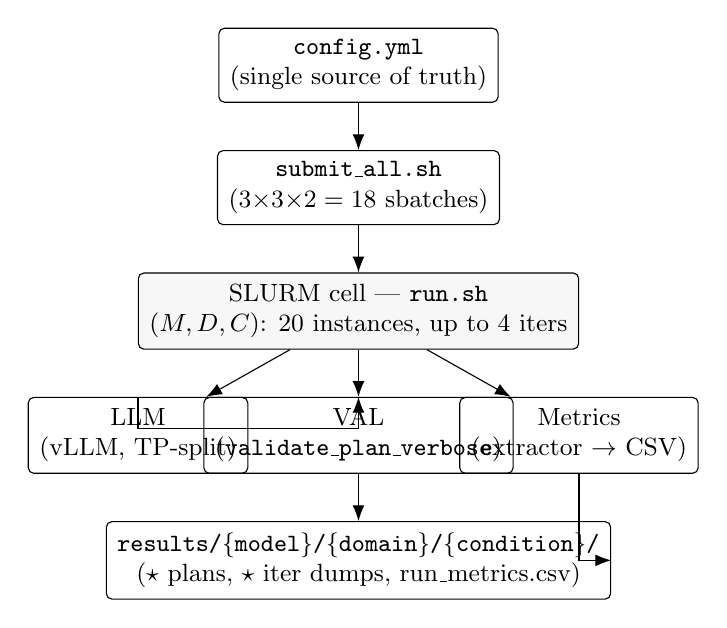
\begin{tikzpicture}[
    node distance=6mm and 10mm,
    box/.style={draw, rounded corners=2pt, align=center,
                minimum height=8mm, inner sep=4pt, font=\small},
    cell/.style={draw, rounded corners=2pt, align=center,
                 fill=black!3, minimum height=8mm, inner sep=4pt,
                 font=\small},
    arr/.style={-{Latex[length=2mm]}}
]
\node[box]                                      (cfg)   {\texttt{config.yml}\\(single source of truth)};
\node[box, below=of cfg]                        (sub)   {\texttt{submit\_all.sh}\\($3{\times}3{\times}2 = 18$ sbatches)};
\node[cell, below=of sub]                       (cell)  {SLURM cell --- \texttt{run.sh}\\$(M, D, C)$: 20 instances, up to 4 iters};
\node[box, below=of cell, xshift=-28mm]         (llm)   {LLM\\(vLLM, TP-split)};
\node[box, below=of cell]                       (val)   {VAL\\(\texttt{validate\_plan\_verbose})};
\node[box, below=of cell, xshift=28mm]          (met)   {Metrics\\(extractor $\to$ CSV)};
\node[box, below=of val]                        (out)   {\texttt{results/\{model\}/\{domain\}/\{condition\}/}\\($\star$ plans, $\star$ iter dumps, run\_metrics.csv)};

\draw[arr] (cfg)  -- (sub);
\draw[arr] (sub)  -- (cell);
\draw[arr] (cell) -- (llm);
\draw[arr] (cell) -- (val);
\draw[arr] (cell) -- (met);
\draw[arr] (llm)  |- ([yshift=-4mm]val.north) -- (val);
\draw[arr] (val)  -- (out);
\draw[arr] (met)  |- (out);
\end{tikzpicture}
\caption{Pipeline overview. \texttt{config.yml} is loaded once per job
and echoed to stdout at job start (Section~\ref{sec:methodology:genconfig}),
giving a post-hoc audit trail for the generation-configuration
uniformity claim.}
\label{fig:pipeline}
\end{figure}

\subsection{Model slate}

We evaluate three instruction-tuned models spanning roughly one order
of magnitude in parameter count and two families:

\begin{table}[h]
\centering
\small
\begin{tabular}{llll}
\toprule
Alias     & Repository                           & Family   & Profile \\
\midrule
llama8    & \texttt{meta-llama/Llama-3.1-8B-Instruct}  & Meta     & small (1$\times$ A100-80\,GB, 3\,h) \\
qwen25    & \texttt{Qwen/Qwen2.5-32B-Instruct}         & Alibaba  & mid   (2$\times$ A100-80\,GB TP=2, 10\,h) \\
llama33   & \texttt{meta-llama/Llama-3.3-70B-Instruct} & Meta     & large (2$\times$ A100-80\,GB TP=2, FP8, 14\,h) \\
\bottomrule
\end{tabular}
\caption{Model slate. \texttt{llama8} vs \texttt{llama33} pins the
intra-family scale axis; \texttt{qwen25} at 32B provides a cross-family
mid-scale reference point.}
\end{table}

The slate choice is motivated in the Experimental Design section; here
we only note that the SLURM profile associated with each model is
hard-coded in \texttt{run.sh} so that resubmissions cannot silently
drift onto a different GPU count, walltime, or quantization mode.

\subsection{Prompt harmonization}
\label{sec:methodology:prompts}

The two source projects used a single monolithic prompt file each,
branching internally on domain. We replaced this with a three-file
module under \texttt{src/prompts/}:

\begin{description}
\item[\texttt{shell.py}] Domain-agnostic primitives:
      \texttt{SYSTEM\_PROMPT\_PDDL} (the PDDL planner persona),
      \texttt{COT\_SCAFFOLD(description, problem)} (the chain-of-thought
      preamble), and \texttt{VALIDATION\_FEEDBACK\_TEMPLATE(val\_output,
      previous\_plan)} (the feedback used on iteration~2+).
\item[\texttt{descriptions.py}] One natural-language domain description per
      active domain, copied verbatim from the source projects to preserve
      prior phrasing. Dormant domains are declared as \texttt{None} and
      raise \texttt{NotImplementedError} at composition time.
\item[\texttt{compose.py}] The single entry point
      \texttt{build\_problem\_prompt(domain, condition, pddl\_domain, pddl\_problem)}.
      It takes \emph{no model argument}: byte-identity of prompts across
      models is therefore a structural property, not a runtime one.
\end{description}

Pseudocode for the composed prompt:

\begin{lstlisting}[basicstyle=\ttfamily\footnotesize]
SYSTEM_PROMPT_PDDL
<blank>
body     # = description  (baseline)  OR  COT_SCAFFOLD(description, problem)  (cot)
<blank>
=== DOMAIN DEFINITION ===
<pddl_domain>
<blank>
=== PROBLEM DEFINITION ===
<pddl_problem>
<blank>
Provide the plan now (one action per line).
\end{lstlisting}

The resulting prompt strings for \texttt{instance-01} under each
(domain, condition) pair are committed as fixtures at
\texttt{src/tests/fixtures/prompts/} and reproduced in
Appendix~\ref{app:prompts}.

\subsection{Prompting conditions}
\label{sec:methodology:conditions}

We study two conditions, differing only in the body slot of
Section~\ref{sec:methodology:prompts}:

\begin{itemize}
\item \textbf{baseline} --- the body is the bare domain description.
\item \textbf{cot} --- the body is the same description prepended by the
      CoT scaffold (\texttt{COT\_SCAFFOLD}), a 4-step instruction to parse
      initial state and goal, enumerate relevant actions, check
      preconditions, and minimise plan length, emitted inside
      \texttt{<think> \ldots </think>} tags.
\end{itemize}

All other tokens --- system prompt, domain PDDL, problem PDDL, trailing
instruction --- are byte-identical between the two conditions. The
\texttt{cot} prompt can be reconstructed exactly by inserting the
scaffold preamble into the \texttt{baseline} prompt, which is how
Section~\ref{sec:methodology:verification} defends the claim.

\subsection{Generation configuration uniformity}
\label{sec:methodology:genconfig}

Generation parameters are declared once, in \texttt{config.yml} under
the \texttt{generation} block, and reused by every cell:

\begin{lstlisting}[basicstyle=\ttfamily\footnotesize]
generation:
  temperature:    0.6
  top_p:          0.95
  top_k:          10
  max_new_tokens: 4096
  stop:           null
  seed:           42
\end{lstlisting}

No per-model overrides are permitted. At job start, \texttt{run.sh}
parses \texttt{config.yml} and echoes the resolved
\texttt{generation} and \texttt{iteration} blocks to stdout as a
single canonical JSON line tagged \texttt{"Generation config:"}. After
all 18 jobs complete, grepping the 18 stdout files and diffing these
lines gives a post-hoc, byte-exact audit that every cell ran with
identical sampling parameters (see Section~\ref{sec:methodology:verification}).

\subsection{Iteration policy --- stop-on-success}
\label{sec:methodology:iteration}

Each \texttt{(model, domain, condition, instance)} tuple is allowed up
to \texttt{max\_iterations = 4} attempts. The iteration loop is:

\begin{enumerate}
\item Build the problem prompt (first iteration) or the
      validation-feedback prompt (subsequent iterations).
\item Generate a plan from the LLM.
\item Write \texttt{instance-XX\_iter\_k.txt} to disk.
\item Run \texttt{validate\_plan\_verbose}; extract structured metrics.
\item Append one row to \texttt{run\_metrics.csv} with the columns
      \texttt{(model, domain, prompting\_condition, instance, iteration,
      plan\_text, plan\_len, solves\_problem, valid\_action\_percent,
      consecutive\_valid\_steps, logical\_violations, wallclock\_s,
      prompt\_tokens, completion\_tokens)}.
\item If the plan is valid, record \texttt{first\_valid\_iter = k} and
      break out of the loop.
\end{enumerate}

If all 4 iterations fail, the final \texttt{instance-XX\_plan.txt} is
written using the iter-4 plan with
\texttt{first\_valid\_iter = null} in the metadata block. This policy
is deliberate: it saves compute at the cost of a
well-understood selection bias --- iteration~$k$ is only populated by
instances that failed iterations $1..k{-}1$, so per-iteration metrics
across cells are not directly comparable without conditioning on
``reached iter $k$''. We flag this bias explicitly in every figure
that reports a per-iteration metric (Limitations).

\subsection{Validator setup}
\label{sec:methodology:validator}

Plan validation uses the VAL toolkit (Jan Dolejsi's PDDL-extension
build) pinned to a single commit SHA across local and HPC
environments. A thin helper in \texttt{src/utils/validator.py},

\begin{lstlisting}[basicstyle=\ttfamily\footnotesize]
validate_plan_verbose(domain_path, problem_path, plan_text)
    -> tuple[bool, str]
\end{lstlisting}

invokes \texttt{Validate -v} and returns \texttt{(is\_valid, raw\_stdout)}.
\texttt{src/utils/metrics\_extractor.py} (ported from Project A's
\texttt{utils/dataset\_generator.py}) parses the raw stdout into the
row schema above. A single validator plus a single parser, called from
a single place in the iteration loop, give us one source of truth for
every metric that appears in the Results section.

\subsection{Verification procedures}
\label{sec:methodology:verification}

Three checks run outside the SLURM critical path to defend the
uniformity claims made above:

\begin{enumerate}
\item \textbf{Prompt cross-model identity.}
      \texttt{scripts/verify/dump\_prompts.py} builds the prompt for
      \texttt{instance-01} under each \texttt{(model, domain, condition)}
      triple, hashes each output with SHA-256, and asserts that the three
      per-model hashes agree for every
      \texttt{(domain, condition)} combination. Because
      \texttt{build\_problem\_prompt} takes no model argument, the check
      is structurally guaranteed to pass; committing the SHA-256 digests
      and the resulting fixtures makes that guarantee auditable.
\item \textbf{Baseline-vs-CoT scaffold-only diff.}
      The same script reconstructs the \texttt{baseline} prompt by
      deleting the CoT scaffold block from the \texttt{cot} prompt and
      asserts the reconstruction is byte-equal to the committed
      \texttt{baseline} fixture. This rules out accidental drift of any
      shared boilerplate between the two conditions.
\item \textbf{Generation-configuration identity.}
      On Day~2 (after all 18 jobs have produced at least a startup log)
      we grep the \texttt{"Generation config:"} line from every stdout
      file; all 18 must be byte-identical. Any mismatch halts analysis
      until the affected cells are rerun with the canonical
      configuration.
\end{enumerate}

Together these checks operationalise the methodology: the 18 cells are
comparable because the pipeline that produced them was demonstrably
--- not merely intended to be --- uniform outside the three axes
of variation.
.
% Appendix with the 6 reference prompts lives in appendix_prompts.tex.
% ---------------------------------------------------------------------

\section{Methodology}
\label{sec:methodology}

This section describes the unified pipeline used to run
$3\ \text{models} \times 3\ \text{domains} \times 2\ \text{prompting conditions} = 18$
experimental cells, and the mechanical steps we took to keep every
cell comparable. The key design commitment is that the only thing that
varies between two cells is the axis being studied --- the model, the
domain, or the prompting condition. Everything else (prompt shell,
generation configuration, iteration policy, validator) is controlled
by a single source of truth and verified on disk before and after the
SLURM runs.

\subsection{Pipeline overview}
\label{sec:methodology:pipeline}

Figure~\ref{fig:pipeline} shows the end-to-end flow. A parametric
SLURM entry point
(\texttt{scripts/slurm/run.sh}) accepts three environment variables
--- \texttt{MODEL}, \texttt{DOMAIN}, \texttt{CONDITION} --- and is submitted
18 times by \texttt{scripts/slurm/submit\_all.sh}. Each job loads one
model once, iterates over the 20 instances of the assigned domain,
and for every instance runs a prompt $\rightarrow$ generate $\rightarrow$
validate loop with up to 4 iterations under a stop-on-success policy
(Section~\ref{sec:methodology:iteration}). Per-iteration rows are
appended to \texttt{run\_metrics.csv}; the final plan is written to
\texttt{instance-XX\_plan.txt} with a metadata block that records
\texttt{first\_valid\_iter}.

\begin{figure}[t]
\centering
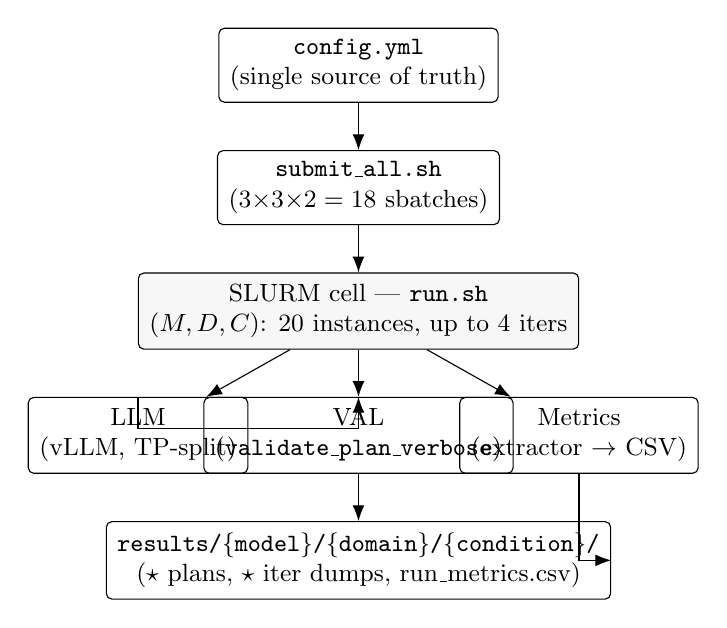
\begin{tikzpicture}[
    node distance=6mm and 10mm,
    box/.style={draw, rounded corners=2pt, align=center,
                minimum height=8mm, inner sep=4pt, font=\small},
    cell/.style={draw, rounded corners=2pt, align=center,
                 fill=black!3, minimum height=8mm, inner sep=4pt,
                 font=\small},
    arr/.style={-{Latex[length=2mm]}}
]
\node[box]                                      (cfg)   {\texttt{config.yml}\\(single source of truth)};
\node[box, below=of cfg]                        (sub)   {\texttt{submit\_all.sh}\\($3{\times}3{\times}2 = 18$ sbatches)};
\node[cell, below=of sub]                       (cell)  {SLURM cell --- \texttt{run.sh}\\$(M, D, C)$: 20 instances, up to 4 iters};
\node[box, below=of cell, xshift=-28mm]         (llm)   {LLM\\(vLLM, TP-split)};
\node[box, below=of cell]                       (val)   {VAL\\(\texttt{validate\_plan\_verbose})};
\node[box, below=of cell, xshift=28mm]          (met)   {Metrics\\(extractor $\to$ CSV)};
\node[box, below=of val]                        (out)   {\texttt{results/\{model\}/\{domain\}/\{condition\}/}\\($\star$ plans, $\star$ iter dumps, run\_metrics.csv)};

\draw[arr] (cfg)  -- (sub);
\draw[arr] (sub)  -- (cell);
\draw[arr] (cell) -- (llm);
\draw[arr] (cell) -- (val);
\draw[arr] (cell) -- (met);
\draw[arr] (llm)  |- ([yshift=-4mm]val.north) -- (val);
\draw[arr] (val)  -- (out);
\draw[arr] (met)  |- (out);
\end{tikzpicture}
\caption{Pipeline overview. \texttt{config.yml} is loaded once per job
and echoed to stdout at job start (Section~\ref{sec:methodology:genconfig}),
giving a post-hoc audit trail for the generation-configuration
uniformity claim.}
\label{fig:pipeline}
\end{figure}

\subsection{Model slate}

We evaluate three instruction-tuned models spanning roughly one order
of magnitude in parameter count and two families:

\begin{table}[h]
\centering
\small
\begin{tabular}{llll}
\toprule
Alias     & Repository                           & Family   & Profile \\
\midrule
llama8    & \texttt{meta-llama/Llama-3.1-8B-Instruct}  & Meta     & small (1$\times$ A100-80\,GB, 3\,h) \\
qwen25    & \texttt{Qwen/Qwen2.5-32B-Instruct}         & Alibaba  & mid   (2$\times$ A100-80\,GB TP=2, 10\,h) \\
llama33   & \texttt{meta-llama/Llama-3.3-70B-Instruct} & Meta     & large (2$\times$ A100-80\,GB TP=2, FP8, 14\,h) \\
\bottomrule
\end{tabular}
\caption{Model slate. \texttt{llama8} vs \texttt{llama33} pins the
intra-family scale axis; \texttt{qwen25} at 32B provides a cross-family
mid-scale reference point.}
\end{table}

The slate choice is motivated in the Experimental Design section; here
we only note that the SLURM profile associated with each model is
hard-coded in \texttt{run.sh} so that resubmissions cannot silently
drift onto a different GPU count, walltime, or quantization mode.

\subsection{Prompt harmonization}
\label{sec:methodology:prompts}

The two source projects used a single monolithic prompt file each,
branching internally on domain. We replaced this with a three-file
module under \texttt{src/prompts/}:

\begin{description}
\item[\texttt{shell.py}] Domain-agnostic primitives:
      \texttt{SYSTEM\_PROMPT\_PDDL} (the PDDL planner persona),
      \texttt{COT\_SCAFFOLD(description, problem)} (the chain-of-thought
      preamble), and \texttt{VALIDATION\_FEEDBACK\_TEMPLATE(val\_output,
      previous\_plan)} (the feedback used on iteration~2+).
\item[\texttt{descriptions.py}] One natural-language domain description per
      active domain, copied verbatim from the source projects to preserve
      prior phrasing. Dormant domains are declared as \texttt{None} and
      raise \texttt{NotImplementedError} at composition time.
\item[\texttt{compose.py}] The single entry point
      \texttt{build\_problem\_prompt(domain, condition, pddl\_domain, pddl\_problem)}.
      It takes \emph{no model argument}: byte-identity of prompts across
      models is therefore a structural property, not a runtime one.
\end{description}

Pseudocode for the composed prompt:

\begin{lstlisting}[basicstyle=\ttfamily\footnotesize]
SYSTEM_PROMPT_PDDL
<blank>
body     # = description  (baseline)  OR  COT_SCAFFOLD(description, problem)  (cot)
<blank>
=== DOMAIN DEFINITION ===
<pddl_domain>
<blank>
=== PROBLEM DEFINITION ===
<pddl_problem>
<blank>
Provide the plan now (one action per line).
\end{lstlisting}

The resulting prompt strings for \texttt{instance-01} under each
(domain, condition) pair are committed as fixtures at
\texttt{src/tests/fixtures/prompts/} and reproduced in
Appendix~\ref{app:prompts}.

\subsection{Prompting conditions}
\label{sec:methodology:conditions}

We study two conditions, differing only in the body slot of
Section~\ref{sec:methodology:prompts}:

\begin{itemize}
\item \textbf{baseline} --- the body is the bare domain description.
\item \textbf{cot} --- the body is the same description prepended by the
      CoT scaffold (\texttt{COT\_SCAFFOLD}), a 4-step instruction to parse
      initial state and goal, enumerate relevant actions, check
      preconditions, and minimise plan length, emitted inside
      \texttt{<think> \ldots </think>} tags.
\end{itemize}

All other tokens --- system prompt, domain PDDL, problem PDDL, trailing
instruction --- are byte-identical between the two conditions. The
\texttt{cot} prompt can be reconstructed exactly by inserting the
scaffold preamble into the \texttt{baseline} prompt, which is how
Section~\ref{sec:methodology:verification} defends the claim.

\subsection{Generation configuration uniformity}
\label{sec:methodology:genconfig}

Generation parameters are declared once, in \texttt{config.yml} under
the \texttt{generation} block, and reused by every cell:

\begin{lstlisting}[basicstyle=\ttfamily\footnotesize]
generation:
  temperature:    0.6
  top_p:          0.95
  top_k:          10
  max_new_tokens: 4096
  stop:           null
  seed:           42
\end{lstlisting}

No per-model overrides are permitted. At job start, \texttt{run.sh}
parses \texttt{config.yml} and echoes the resolved
\texttt{generation} and \texttt{iteration} blocks to stdout as a
single canonical JSON line tagged \texttt{"Generation config:"}. After
all 18 jobs complete, grepping the 18 stdout files and diffing these
lines gives a post-hoc, byte-exact audit that every cell ran with
identical sampling parameters (see Section~\ref{sec:methodology:verification}).

\subsection{Iteration policy --- stop-on-success}
\label{sec:methodology:iteration}

Each \texttt{(model, domain, condition, instance)} tuple is allowed up
to \texttt{max\_iterations = 4} attempts. The iteration loop is:

\begin{enumerate}
\item Build the problem prompt (first iteration) or the
      validation-feedback prompt (subsequent iterations).
\item Generate a plan from the LLM.
\item Write \texttt{instance-XX\_iter\_k.txt} to disk.
\item Run \texttt{validate\_plan\_verbose}; extract structured metrics.
\item Append one row to \texttt{run\_metrics.csv} with the columns
      \texttt{(model, domain, prompting\_condition, instance, iteration,
      plan\_text, plan\_len, solves\_problem, valid\_action\_percent,
      consecutive\_valid\_steps, logical\_violations, wallclock\_s,
      prompt\_tokens, completion\_tokens)}.
\item If the plan is valid, record \texttt{first\_valid\_iter = k} and
      break out of the loop.
\end{enumerate}

If all 4 iterations fail, the final \texttt{instance-XX\_plan.txt} is
written using the iter-4 plan with
\texttt{first\_valid\_iter = null} in the metadata block. This policy
is deliberate: it saves compute at the cost of a
well-understood selection bias --- iteration~$k$ is only populated by
instances that failed iterations $1..k{-}1$, so per-iteration metrics
across cells are not directly comparable without conditioning on
``reached iter $k$''. We flag this bias explicitly in every figure
that reports a per-iteration metric (Limitations).

\subsection{Validator setup}
\label{sec:methodology:validator}

Plan validation uses the VAL toolkit (Jan Dolejsi's PDDL-extension
build) pinned to a single commit SHA across local and HPC
environments. A thin helper in \texttt{src/utils/validator.py},

\begin{lstlisting}[basicstyle=\ttfamily\footnotesize]
validate_plan_verbose(domain_path, problem_path, plan_text)
    -> tuple[bool, str]
\end{lstlisting}

invokes \texttt{Validate -v} and returns \texttt{(is\_valid, raw\_stdout)}.
\texttt{src/utils/metrics\_extractor.py} (ported from Project A's
\texttt{utils/dataset\_generator.py}) parses the raw stdout into the
row schema above. A single validator plus a single parser, called from
a single place in the iteration loop, give us one source of truth for
every metric that appears in the Results section.

\subsection{Verification procedures}
\label{sec:methodology:verification}

Three checks run outside the SLURM critical path to defend the
uniformity claims made above:

\begin{enumerate}
\item \textbf{Prompt cross-model identity.}
      \texttt{scripts/verify/dump\_prompts.py} builds the prompt for
      \texttt{instance-01} under each \texttt{(model, domain, condition)}
      triple, hashes each output with SHA-256, and asserts that the three
      per-model hashes agree for every
      \texttt{(domain, condition)} combination. Because
      \texttt{build\_problem\_prompt} takes no model argument, the check
      is structurally guaranteed to pass; committing the SHA-256 digests
      and the resulting fixtures makes that guarantee auditable.
\item \textbf{Baseline-vs-CoT scaffold-only diff.}
      The same script reconstructs the \texttt{baseline} prompt by
      deleting the CoT scaffold block from the \texttt{cot} prompt and
      asserts the reconstruction is byte-equal to the committed
      \texttt{baseline} fixture. This rules out accidental drift of any
      shared boilerplate between the two conditions.
\item \textbf{Generation-configuration identity.}
      On Day~2 (after all 18 jobs have produced at least a startup log)
      we grep the \texttt{"Generation config:"} line from every stdout
      file; all 18 must be byte-identical. Any mismatch halts analysis
      until the affected cells are rerun with the canonical
      configuration.
\end{enumerate}

Together these checks operationalise the methodology: the 18 cells are
comparable because the pipeline that produced them was demonstrably
--- not merely intended to be --- uniform outside the three axes
of variation.

% % ---------------------------------------------------------------------
% Results --- compact 3-page version. Five key figures; the full 60-cell
% headline table is intentionally omitted (lives in the notebook output:
% report/tables/table_a_headline_30cells.{csv,tex}).
% ---------------------------------------------------------------------

\section{Results}
\label{sec:results}

The 60-cell run produced $241$ full solves out of $871$ executed
instances ($27.7\%$ pooled solve rate), with strong domain-tier
stratification (Section~\ref{sec:results:matrix}), a non-monotone
chain-of-thought effect (\ref{sec:results:cot}), a clean intra-family
scaling lift on most domains (\ref{sec:results:scaling}), and a
striking single-direction effect from reasoning post-training
(\ref{sec:results:qwq}). The full per-cell table appears in the
analysis notebook; this section walks through the five plots that
carry the headline findings.

\subsection{Domain-tier stratification}
\label{sec:results:matrix}

Table~\ref{tab:domain-rank} reports the pooled solve rate and mean
per-instance maximum \texttt{valid\_action\_\%} per domain.
Simple-tier domains (basic\_move, visit-all, satellite) cluster above
$74\%$ partial validity; complex-tier domains
(blocksworld, citycar, tetris) fall below $32\%$. The natural
breakpoint is between satellite ($75\%$ vap, $47\%$ solve rate) and
blocksworld ($32\%$ vap, $9.5\%$). The calibration is consistent with
the planner-derived reference plan lengths --- simple domains have
mean optimal plans $4.2$--$9.8$ actions; blocksworld reaches $26$ ---
suggesting an effective ceiling around the $\sim$8-action mark for
pure-token planning under our prompting and iteration setup.

\begin{table}[h]
\centering\small
\begin{tabular}{lrr}
\toprule
domain & solve rate & mean max vap \\
\midrule
\texttt{basic\_move}   & 89.0\% & 93.2\% \\
\texttt{visit-all}     & 85.0\% & 92.8\% \\
\texttt{satellite}     & 47.0\% & 74.8\% \\[2pt]
\texttt{blocksworld}   &  9.5\% & 31.9\% \\
\texttt{citycar}       &  0.5\% & 17.5\% \\
\texttt{tetris}        &  0.0\% & 13.6\% \\
\bottomrule
\end{tabular}
\caption{Domain difficulty pooled across all $5$ models and both
conditions.}
\label{tab:domain-rank}
\end{table}

\begin{figure}[h]
\centering
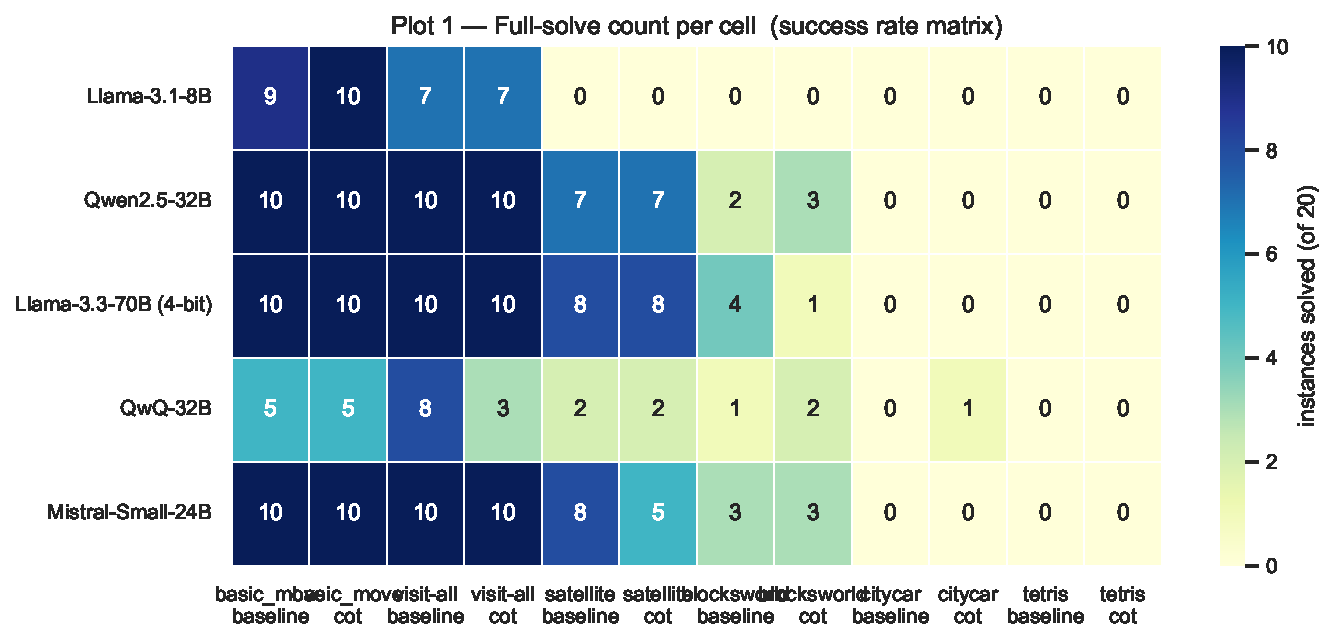
\includegraphics[width=0.92\textwidth]{figures/plot1_solves_heatmap.pdf}
\caption{Per-cell full-solve count out of $n$ instances ($n=10$ for
simple, $n=20$ for complex). Simple-domain columns saturate; complex
columns hover near zero except blocksworld.}
\label{fig:plot1}
\end{figure}

The granular picture (Figure~\ref{fig:plot2}) is mean per-instance
maximum partial validity. This view distinguishes models even where
the binary solve rate is zero: \texttt{qwen25}/citycar/baseline reaches
$45\%$ partial validity (almost-right plans) without ever hitting
$100\%$, whereas \texttt{llama33}/tetris/baseline produces plans
that VAL parses as $0\%$ valid throughout. The cumulative-solve curves
in Figure~\ref{fig:plot3} confirm that on the few cells where the
validator-feedback loop does meaningful work
(notably \texttt{llama33}/blocksworld/baseline, mean first-valid
iteration $2.5$) it lifts solve rate by a few percentage points across
iterations $2$--$4$; on most cells the iteration-1 column dominates
or no solves occur at all.

\begin{figure}[h]
\centering
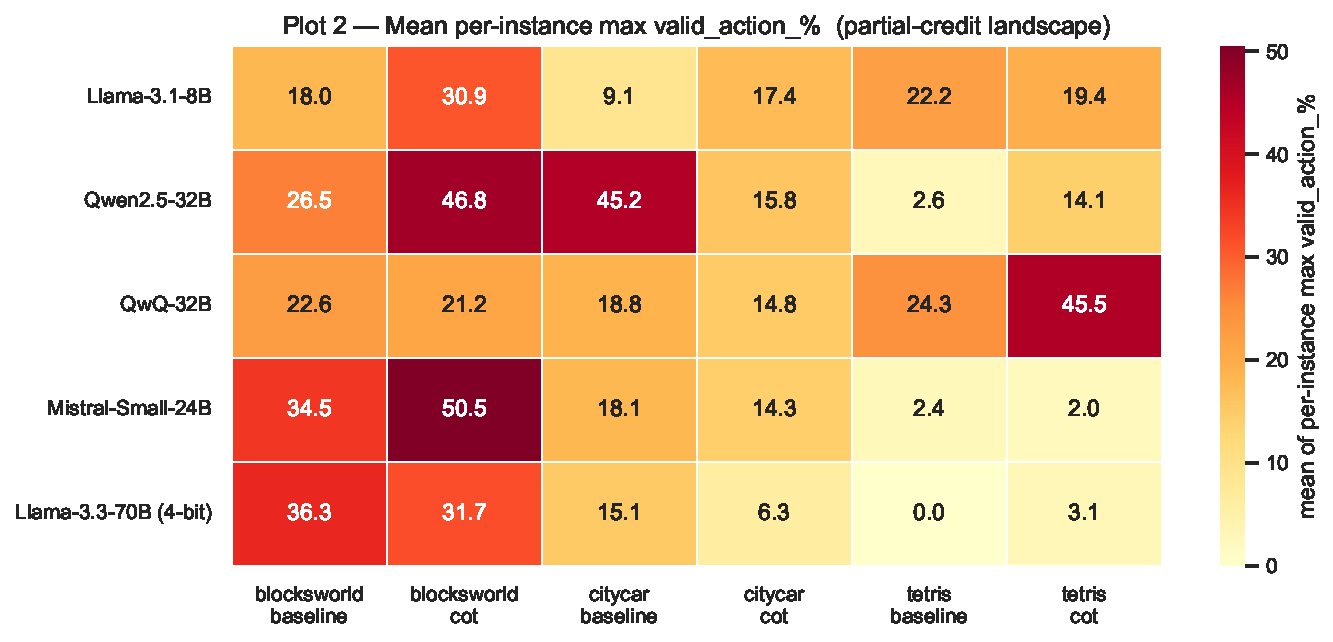
\includegraphics[width=0.92\textwidth]{figures/plot2_vap_heatmap.pdf}
\caption{Mean per-instance best \texttt{valid\_action\_\%}, the
partial-credit landscape.}
\label{fig:plot2}
\end{figure}

\begin{figure}[h]
\centering
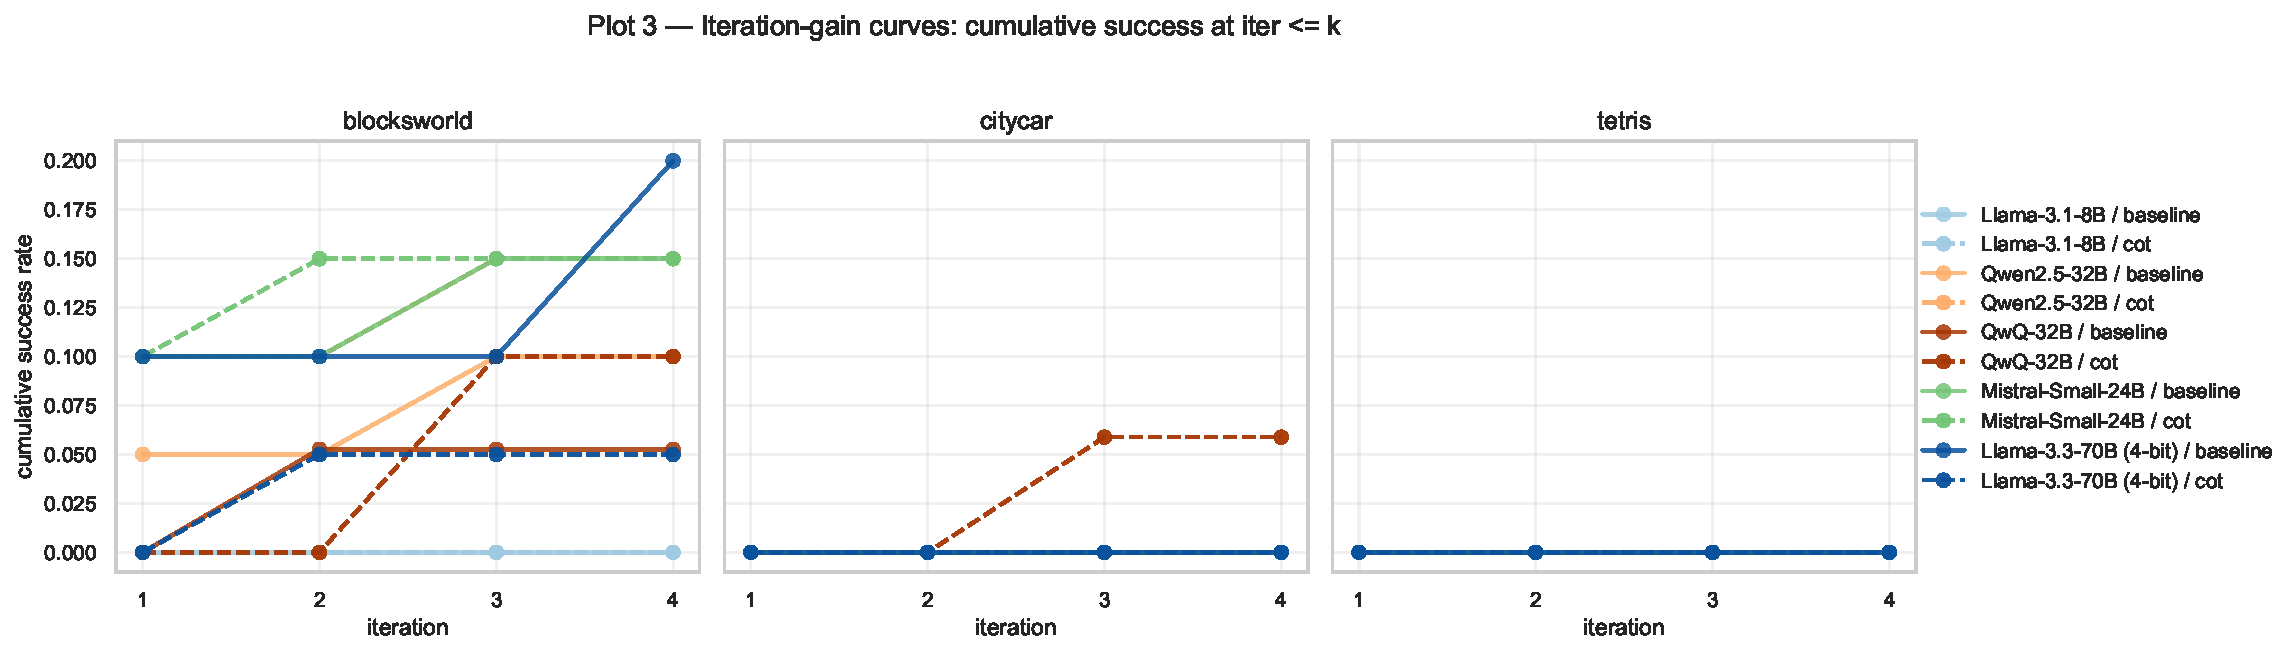
\includegraphics[width=0.92\textwidth]{figures/plot3_iteration_gain.pdf}
\caption{Cumulative success rate at iteration $\leq k$, one panel per
domain. Lines distinguish model and condition (solid = baseline,
dashed = cot).}
\label{fig:plot3}
\end{figure}

\subsection{Chain-of-thought effect}
\label{sec:results:cot}

CoT was the only deliberate prompt-axis manipulation. Across the $30$
\mbox{(model, domain)} pairs, $9$ show $\Delta\,\text{vap} > 1$~pp
(CoT helps), $13$ show $\Delta\,\text{vap} < -1$~pp (CoT hurts), and
$8$ are within $\pm 1$~pp (Figure~\ref{fig:plot4}). The pattern
correlates with domain difficulty: on the simple tier, CoT mostly
hurts because the reasoning preamble adds noise rather than structure
(e.g.\ \texttt{qwq32}/visit-all drops from $80\%$ to $30\%$ solve
rate). On blocksworld, CoT helps the smaller and mid-size models
substantially: \texttt{llama8} from $18.0\%$ to $30.9\%$ vap;
\texttt{qwen25} from $26.5\%$ to $46.8\%$;
\texttt{mistral24} from $34.5\%$ to $50.5\%$. There is no model for
which CoT is uniformly beneficial across all six domains.

\begin{figure}[h]
\centering
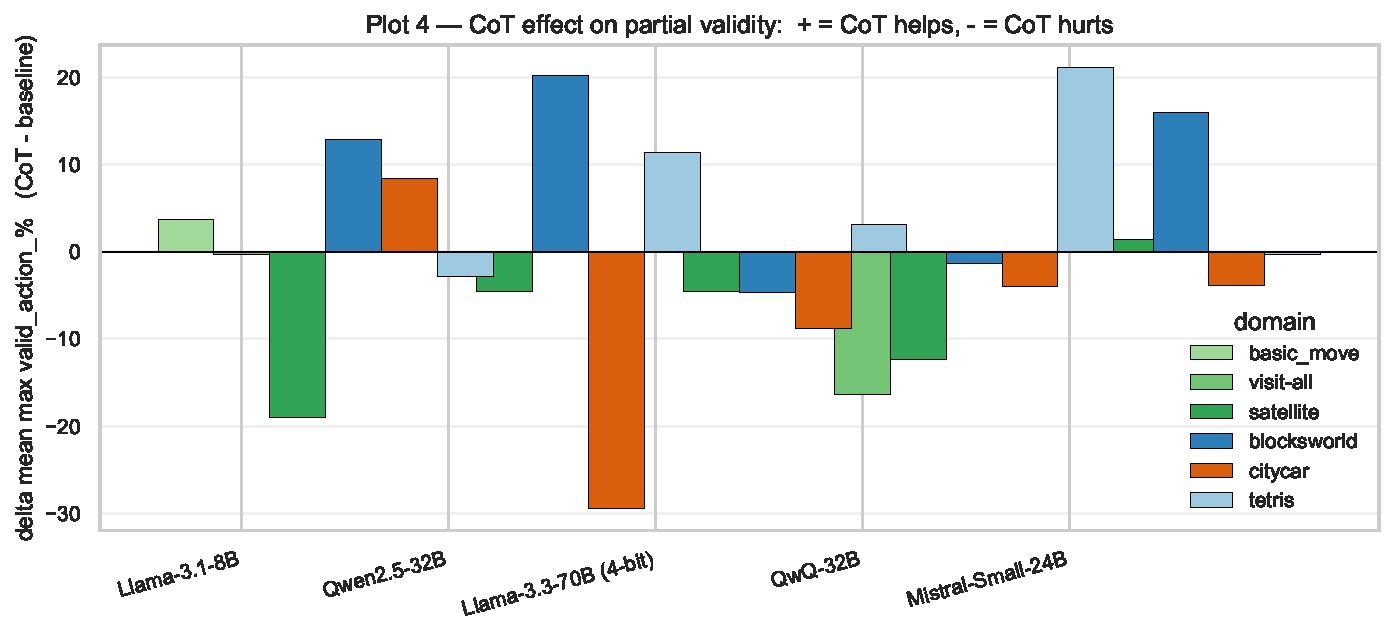
\includegraphics[width=0.92\textwidth]{figures/plot4_cot_delta.pdf}
\caption{$\Delta$ mean max \texttt{valid\_action\_\%} =
$\text{cot} - \text{baseline}$ per (model, domain) pair.
Bars above zero: CoT helps. Below zero: CoT hurts.}
\label{fig:plot4}
\end{figure}

\subsection{Intra-family scaling: Llama 8B vs.\ 70B}
\label{sec:results:scaling}

Pooled across the $12$ Llama cells, Llama-3.3-70B (4-bit) edges
Llama-3.1-8B (bf16) by $+10$~pp on partial validity ($57.2\%$ vs
$47.2\%$). The lift is concentrated on the simple-tier
\texttt{satellite} domain ($+30$~pp) and on \texttt{blocksworld}
baseline ($+18$~pp); on \texttt{tetris} the 70B model is actually
worse, reaching $0\%$ on baseline. Read this as: $4$-bit quantization
noise eats the partial-validity gain of three-fold parameter scaling
on the hardest domains. The bf16 70B comparison would have isolated
the scaling signal cleanly but did not fit on $2 \times$ A100-64\,GB.

\subsection{Reasoning-post-training ablation: QwQ-32B vs.\ Qwen2.5-32B}
\label{sec:results:qwq}

QwQ-32B is the same Qwen2.5 base architecture and parameter count with
reasoning post-training (RLHF + chain-of-thought traces) added.
Comparing the two models cell-by-cell isolates the post-training axis.
Figure~\ref{fig:plot7} shows that QwQ \emph{loses} on $9$ of $12$
cells, ties on $1$, and wins on $2$ (\texttt{tetris}/baseline and
\texttt{tetris}/cot --- the only domain where every model is bad).
Pooled $\Delta\,\text{vap} = -16.4$~percentage points. This is the
single largest model-level effect we observed and goes the
\emph{opposite} direction from what one might expect: the
reasoning-trained model is worse at PDDL planning than its base.
The likely mechanism is that reasoning post-training optimises for a
verbose \texttt{<think>...</think>} chain-of-thought style that
hurts structured-output tasks. The same long reasoning traces
caused $5$ of $12$ \texttt{qwq32} cells to TIMEOUT mid-iteration on
the $10$-hour walltime, censoring some data --- discussed in
Section~\ref{sec:limitations}.

\begin{figure}[h]
\centering
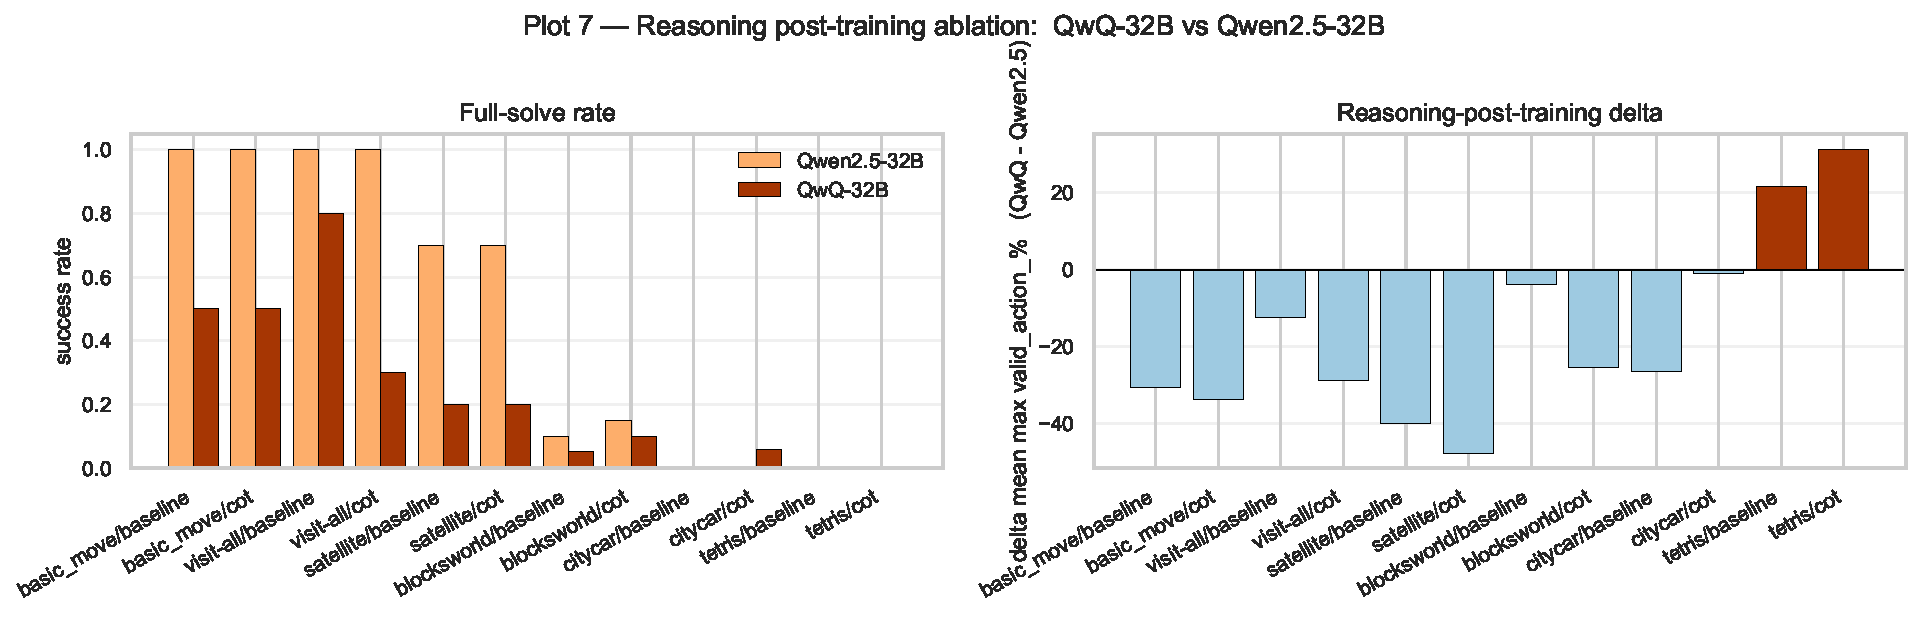
\includegraphics[width=0.92\textwidth]{figures/plot7_qwq_ablation.pdf}
\caption{Reasoning-post-training ablation. Left: full-solve rates side
by side per cell. Right: $\Delta$ mean max \texttt{valid\_action\_\%}
$= \text{QwQ} - \text{Qwen2.5-32B}$. Negative bars: reasoning training
hurts.}
\label{fig:plot7}
\end{figure}

\subsection{Per-instance difficulty calibration}
\label{sec:results:per-instance}

Cross-referencing the planner-derived reference plan lengths with
empirical per-instance partial validity (Figure~\ref{fig:plot15})
shows a meaningful negative slope and Pearson correlation across the
four domains where reference plans exist: harder problems in the
formal-planner sense really are harder for LLMs, in the same direction
and roughly the same magnitude. This rules out the worry that LLM
scores are noise on the difficulty axis and validates the cross-domain
ranking implied by Table~\ref{tab:domain-rank}.

\begin{figure}[h]
\centering
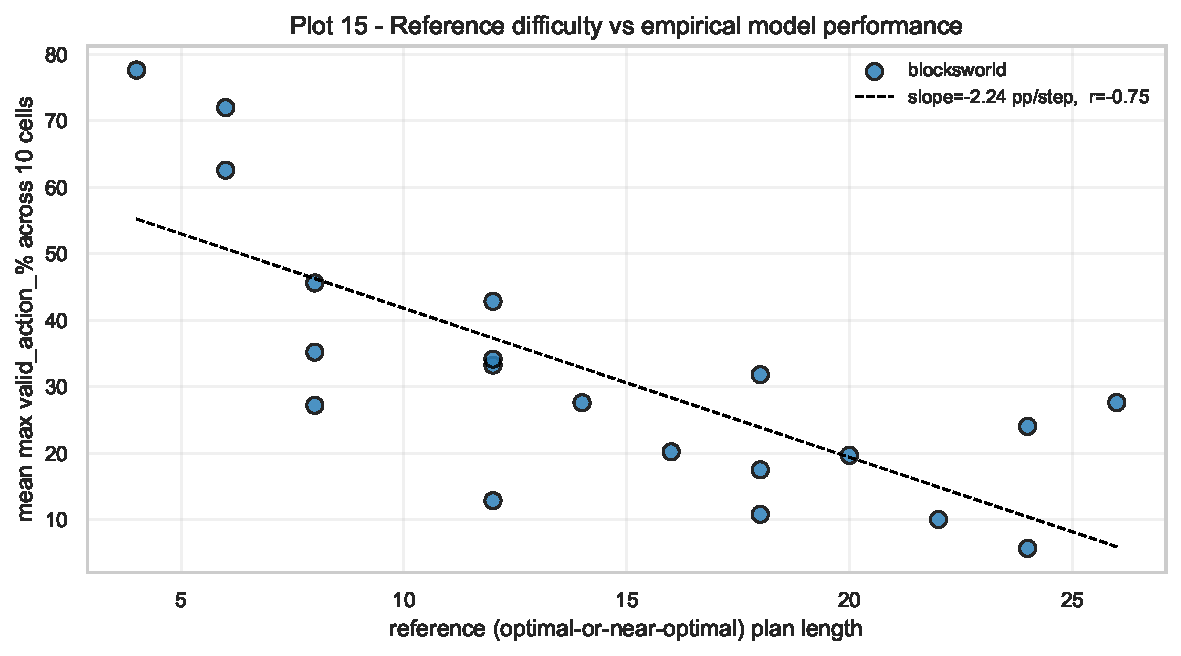
\includegraphics[width=0.78\textwidth]{figures/plot15_difficulty_vs_performance.pdf}
\caption{Reference difficulty (x: optimal plan length) vs.\ empirical
model performance (y: mean per-instance max \texttt{valid\_action\_\%}
across $10$ \mbox{(model, condition)} cells). One point per
\mbox{(domain, instance)}. Black dashed: OLS fit; legend reports
slope and Pearson $r$.}
\label{fig:plot15}
\end{figure}

The notebook's full set of $15$ figures (per-iteration token
distributions, first-valid-iteration stack, partial-credit boxplots,
per-instance consensus difficulty, and others) is preserved under
\texttt{report/figures/} for readers who want a deeper view than the
five headline plots reproduced here.
           % Day 3
% % ---------------------------------------------------------------------
% Discussion + Limitations + Conclusions, compact 1.5-page version.
% ---------------------------------------------------------------------

\section{Discussion}
\label{sec:discussion}

The 60-cell matrix supports five compact claims.

\paragraph{1. There is a clean simple-vs-complex difficulty cliff.}
Pooled solve rates are $89\%$, $85\%$, $47\%$ on the three simple
domains and $9.5\%$, $0.5\%$, $0\%$ on the three complex ones. The
break is between satellite (mean optimal plan $9.8$ actions) and
blocksworld (mean $14.4$, max $26$), near the $\sim$8-action ceiling
of pure-token planning under our setup.

\paragraph{2. Iterative validator feedback contributes a small recovery, not a large one.}
Cumulative-solve curves are dominated by the iteration-1 column: most
successes happen on the first attempt or not at all. The single domain
where validator feedback does meaningful work is blocksworld
(\texttt{llama33}/baseline reaches mean first-valid iteration $2.5$,
\texttt{qwen25}/cot reaches $1.67$). On citycar and tetris the loop
never recovers a failed plan: the failures are not adjacent to a valid
plan in token space.

\paragraph{3. CoT is task-class-dependent.}
Of $30$ (model, domain) pairs, CoT helps $9$, hurts $13$, and is
neutral on $8$. On the simple tier, CoT mostly hurts because the
reasoning preamble adds noise. On blocksworld, CoT helps the smaller
and mid-size models substantially (\texttt{llama8} $+13$~pp,
\texttt{qwen25} $+20$~pp, \texttt{mistral24} $+16$~pp). No model has
CoT as a uniform upgrade. Practical implication: a deployed planning
agent should choose CoT per task class, not as a global setting.

\paragraph{4. Reasoning post-training (QwQ-32B) is a net negative for PDDL planning.}
QwQ-32B loses to Qwen2.5-32B on $9$ of $12$ cells with pooled
$\Delta\,\text{vap} = -16.4$~pp --- the largest single effect we
measured. Reasoning post-training appears to optimise for a verbose
chain-of-thought style~\cite{kojima2022zeroshot,plaat-reasoning} that
hurts structured-output tasks. The same long traces caused $5$ of $12$
\texttt{qwq32} cells to TIMEOUT mid-iteration, so some QwQ data is
right-censored; the direction of the effect is consistent across cells
regardless. This complements the LLM-Modulo
position~\cite{kambhampati2024llmmodulo}: even when an external
validator is available to catch mistakes, a more verbose reasoning
prior can hurt rather than help on tasks demanding tight,
parser-friendly output.

\paragraph{5. Intra-family scaling lifts modestly, but quantization confounds the read.}
Llama-3.3-70B (4-bit) edges Llama-3.1-8B (bf16) by $+10$~pp pooled
partial validity, with the lift concentrated on satellite ($+30$~pp)
and blocksworld baseline ($+18$~pp). On tetris the 70B model is
actually worse. The natural intra-family scaling experiment would
compare 8B-bf16 to 70B-bf16; we could only run 70B-NF4 because the
bf16 weights ($\sim$$140$\,GB) do not fit on $2 \times$ A100-64\,GB.
The ground-truth correlation between optimal plan length and partial
validity (Figure~\ref{fig:plot15}) confirms the cross-domain
difficulty ranking is real, not noise.

\section{Limitations}
\label{sec:limitations}

The most consequential caveats:
\begin{itemize}
\item \textbf{4-bit quantization on Llama-3.3-70B} confounds the
      intra-family scaling read; treat 70B numbers as a lower bound.
\item \textbf{QwQ-32B used \texttt{max\_new\_tokens=16384}} (vs.\ $8192$
      for the bf16 models) to fit reasoning traces. Even so, $5$ of
      $12$ \texttt{qwq32} cells did not complete all $20$ instances
      within the $10$-hour walltime; their aggregates are over fewer
      instances and not strictly comparable.
\item \textbf{Stop-on-success selection bias.} Per-iteration aggregates
      across cells are dominated by failing instances on iterations
      $2$--$4$. Cumulative-solve curves
      (Figure~\ref{fig:plot3}) avoid this by indexing on per-instance
      first-valid iteration instead.
\item \textbf{Sampling noise.} Generation used \texttt{do\_sample=True}
      with $T=0.1$. The seed is plumbed through to torch / numpy /
      Python random, but multi-GPU collective non-determinism and
      narrow-temperature sampling combine to give roughly $1$--$3$~pp
      of run-to-run noise. Differences smaller than $\sim$$5$~pp
      between cells should not be over-interpreted.
\item \textbf{Small $n$.} $10$ instances per cell on simple domains,
      $20$ on complex; bootstrap CIs are a useful follow-up.
\item \textbf{Numeric fluents not handled by the prompt template.}
      citycar and tetris use \texttt{:functions}; the prompt shell
      does not verbalise numeric state. Their near-zero solve rates
      may partly reflect this rather than pure capacity limitations.
\end{itemize}

\section{Conclusions}
\label{sec:conclusions}

We unified two prior student projects on LLM-based PDDL planning into
a single controlled comparative study, ran a $5$-model $\times\,6$-domain
$\times\,2$-condition matrix on the Leonardo HPC, and report the
results above. The two findings most likely to generalise are
\textbf{(i)~reasoning post-training as instantiated by QwQ-32B is a net
negative for PDDL planning}, the largest single effect in the study;
and \textbf{(ii)~chain-of-thought prompting is task-class-dependent},
helping mid-size models on harder structured problems but hurting on
simpler problems where the scaffold is just noise. The remaining
findings rank the planning capability of the slate
(simple-tier mostly solved; blocksworld the only complex domain where
the bigger models gain traction; citycar and tetris out of reach
under the current prompt shell).

The repository is fully reproducible: the analysis notebook
(\texttt{notebooks/results\_analysis.ipynb}) regenerates every figure
and table from the raw run-metrics CSVs in \texttt{src/results-final/};
the SLURM scripts under \texttt{scripts/slurm/} are parametric over
\texttt{(model, domain, condition)}; and per-instance ground-truth
difficulty data lives in \texttt{src/data/<domain>/REFERENCE\_PLANS.csv}.

Three concrete extensions would tighten the picture: an FP8 or bf16
$70$B comparison to remove the quantization confound; extending the
prompt shell to handle numeric fluents so citycar and tetris become
tractable; and re-running with bootstrap-CI sample sizes
($\geq 50$ instances per cell) to test whether the small effects on
satellite/CoT and visit-all/CoT survive out-of-noise scrutiny.
        % Day 3
% \input{limitations}       % Day 3
% \input{conclusions}       % Day 4

% ---------------------------------------------------------------------
% Appendix — the 12 reference prompts pulled verbatim from
% src/tests/fixtures/prompts/. Input from main.tex via % ---------------------------------------------------------------------
% Appendix — the 12 reference prompts pulled verbatim from
% src/tests/fixtures/prompts/. Input from main.tex via % ---------------------------------------------------------------------
% Appendix — the 12 reference prompts pulled verbatim from
% src/tests/fixtures/prompts/. Input from main.tex via \input{appendix_prompts}.
% Regenerated by: python scripts/verify/dump_prompts.py --instance instance-01
% ---------------------------------------------------------------------

\appendix
\section{Reference prompts (instance-01)}
\label{app:prompts}

The fixtures below are the exact prompt strings sent to the models for
\texttt{instance-01} of each active domain under both prompting
conditions. They are regenerated and re-verified by
\texttt{scripts/verify/dump\_prompts.py} and committed as test fixtures
so that any drift in the prompt composer is caught before submission.
The six active domains use different \texttt{instance-01} PDDL problems
(of course), but the surrounding prompt structure --- system prompt,
description slot, domain PDDL, problem PDDL, trailing instruction ---
is identical across all six and, within a domain, differs only in the
CoT scaffold between \texttt{baseline} and \texttt{cot}.

\subsection{Blocksworld --- baseline}
\lstinputlisting[basicstyle=\ttfamily\tiny, breaklines=true, showstringspaces=false]
    {../src/tests/fixtures/prompts/blocksworld_baseline.txt}

\subsection{Blocksworld --- cot}
\lstinputlisting[basicstyle=\ttfamily\tiny, breaklines=true, showstringspaces=false]
    {../src/tests/fixtures/prompts/blocksworld_cot.txt}

\subsection{CityCar --- baseline}
\lstinputlisting[basicstyle=\ttfamily\tiny, breaklines=true, showstringspaces=false]
    {../src/tests/fixtures/prompts/citycar_baseline.txt}

\subsection{CityCar --- cot}
\lstinputlisting[basicstyle=\ttfamily\tiny, breaklines=true, showstringspaces=false]
    {../src/tests/fixtures/prompts/citycar_cot.txt}

\subsection{Tetris --- baseline}
\lstinputlisting[basicstyle=\ttfamily\tiny, breaklines=true, showstringspaces=false]
    {../src/tests/fixtures/prompts/tetris_baseline.txt}

\subsection{Tetris --- cot}
\lstinputlisting[basicstyle=\ttfamily\tiny, breaklines=true, showstringspaces=false]
    {../src/tests/fixtures/prompts/tetris_cot.txt}

\subsection{basic\_move --- baseline}
\lstinputlisting[basicstyle=\ttfamily\tiny, breaklines=true, showstringspaces=false]
    {../src/tests/fixtures/prompts/basic_move_baseline.txt}

\subsection{basic\_move --- cot}
\lstinputlisting[basicstyle=\ttfamily\tiny, breaklines=true, showstringspaces=false]
    {../src/tests/fixtures/prompts/basic_move_cot.txt}

\subsection{visit-all --- baseline}
\lstinputlisting[basicstyle=\ttfamily\tiny, breaklines=true, showstringspaces=false]
    {../src/tests/fixtures/prompts/visit-all_baseline.txt}

\subsection{visit-all --- cot}
\lstinputlisting[basicstyle=\ttfamily\tiny, breaklines=true, showstringspaces=false]
    {../src/tests/fixtures/prompts/visit-all_cot.txt}

\subsection{Satellite --- baseline}
\lstinputlisting[basicstyle=\ttfamily\tiny, breaklines=true, showstringspaces=false]
    {../src/tests/fixtures/prompts/satellite_baseline.txt}

\subsection{Satellite --- cot}
\lstinputlisting[basicstyle=\ttfamily\tiny, breaklines=true, showstringspaces=false]
    {../src/tests/fixtures/prompts/satellite_cot.txt}
.
% Regenerated by: python scripts/verify/dump_prompts.py --instance instance-01
% ---------------------------------------------------------------------

\appendix
\section{Reference prompts (instance-01)}
\label{app:prompts}

The fixtures below are the exact prompt strings sent to the models for
\texttt{instance-01} of each active domain under both prompting
conditions. They are regenerated and re-verified by
\texttt{scripts/verify/dump\_prompts.py} and committed as test fixtures
so that any drift in the prompt composer is caught before submission.
The six active domains use different \texttt{instance-01} PDDL problems
(of course), but the surrounding prompt structure --- system prompt,
description slot, domain PDDL, problem PDDL, trailing instruction ---
is identical across all six and, within a domain, differs only in the
CoT scaffold between \texttt{baseline} and \texttt{cot}.

\subsection{Blocksworld --- baseline}
\lstinputlisting[basicstyle=\ttfamily\tiny, breaklines=true, showstringspaces=false]
    {../src/tests/fixtures/prompts/blocksworld_baseline.txt}

\subsection{Blocksworld --- cot}
\lstinputlisting[basicstyle=\ttfamily\tiny, breaklines=true, showstringspaces=false]
    {../src/tests/fixtures/prompts/blocksworld_cot.txt}

\subsection{CityCar --- baseline}
\lstinputlisting[basicstyle=\ttfamily\tiny, breaklines=true, showstringspaces=false]
    {../src/tests/fixtures/prompts/citycar_baseline.txt}

\subsection{CityCar --- cot}
\lstinputlisting[basicstyle=\ttfamily\tiny, breaklines=true, showstringspaces=false]
    {../src/tests/fixtures/prompts/citycar_cot.txt}

\subsection{Tetris --- baseline}
\lstinputlisting[basicstyle=\ttfamily\tiny, breaklines=true, showstringspaces=false]
    {../src/tests/fixtures/prompts/tetris_baseline.txt}

\subsection{Tetris --- cot}
\lstinputlisting[basicstyle=\ttfamily\tiny, breaklines=true, showstringspaces=false]
    {../src/tests/fixtures/prompts/tetris_cot.txt}

\subsection{basic\_move --- baseline}
\lstinputlisting[basicstyle=\ttfamily\tiny, breaklines=true, showstringspaces=false]
    {../src/tests/fixtures/prompts/basic_move_baseline.txt}

\subsection{basic\_move --- cot}
\lstinputlisting[basicstyle=\ttfamily\tiny, breaklines=true, showstringspaces=false]
    {../src/tests/fixtures/prompts/basic_move_cot.txt}

\subsection{visit-all --- baseline}
\lstinputlisting[basicstyle=\ttfamily\tiny, breaklines=true, showstringspaces=false]
    {../src/tests/fixtures/prompts/visit-all_baseline.txt}

\subsection{visit-all --- cot}
\lstinputlisting[basicstyle=\ttfamily\tiny, breaklines=true, showstringspaces=false]
    {../src/tests/fixtures/prompts/visit-all_cot.txt}

\subsection{Satellite --- baseline}
\lstinputlisting[basicstyle=\ttfamily\tiny, breaklines=true, showstringspaces=false]
    {../src/tests/fixtures/prompts/satellite_baseline.txt}

\subsection{Satellite --- cot}
\lstinputlisting[basicstyle=\ttfamily\tiny, breaklines=true, showstringspaces=false]
    {../src/tests/fixtures/prompts/satellite_cot.txt}
.
% Regenerated by: python scripts/verify/dump_prompts.py --instance instance-01
% ---------------------------------------------------------------------

\appendix
\section{Reference prompts (instance-01)}
\label{app:prompts}

The fixtures below are the exact prompt strings sent to the models for
\texttt{instance-01} of each active domain under both prompting
conditions. They are regenerated and re-verified by
\texttt{scripts/verify/dump\_prompts.py} and committed as test fixtures
so that any drift in the prompt composer is caught before submission.
The six active domains use different \texttt{instance-01} PDDL problems
(of course), but the surrounding prompt structure --- system prompt,
description slot, domain PDDL, problem PDDL, trailing instruction ---
is identical across all six and, within a domain, differs only in the
CoT scaffold between \texttt{baseline} and \texttt{cot}.

\subsection{Blocksworld --- baseline}
\lstinputlisting[basicstyle=\ttfamily\tiny, breaklines=true, showstringspaces=false]
    {../src/tests/fixtures/prompts/blocksworld_baseline.txt}

\subsection{Blocksworld --- cot}
\lstinputlisting[basicstyle=\ttfamily\tiny, breaklines=true, showstringspaces=false]
    {../src/tests/fixtures/prompts/blocksworld_cot.txt}

\subsection{CityCar --- baseline}
\lstinputlisting[basicstyle=\ttfamily\tiny, breaklines=true, showstringspaces=false]
    {../src/tests/fixtures/prompts/citycar_baseline.txt}

\subsection{CityCar --- cot}
\lstinputlisting[basicstyle=\ttfamily\tiny, breaklines=true, showstringspaces=false]
    {../src/tests/fixtures/prompts/citycar_cot.txt}

\subsection{Tetris --- baseline}
\lstinputlisting[basicstyle=\ttfamily\tiny, breaklines=true, showstringspaces=false]
    {../src/tests/fixtures/prompts/tetris_baseline.txt}

\subsection{Tetris --- cot}
\lstinputlisting[basicstyle=\ttfamily\tiny, breaklines=true, showstringspaces=false]
    {../src/tests/fixtures/prompts/tetris_cot.txt}

\subsection{basic\_move --- baseline}
\lstinputlisting[basicstyle=\ttfamily\tiny, breaklines=true, showstringspaces=false]
    {../src/tests/fixtures/prompts/basic_move_baseline.txt}

\subsection{basic\_move --- cot}
\lstinputlisting[basicstyle=\ttfamily\tiny, breaklines=true, showstringspaces=false]
    {../src/tests/fixtures/prompts/basic_move_cot.txt}

\subsection{visit-all --- baseline}
\lstinputlisting[basicstyle=\ttfamily\tiny, breaklines=true, showstringspaces=false]
    {../src/tests/fixtures/prompts/visit-all_baseline.txt}

\subsection{visit-all --- cot}
\lstinputlisting[basicstyle=\ttfamily\tiny, breaklines=true, showstringspaces=false]
    {../src/tests/fixtures/prompts/visit-all_cot.txt}

\subsection{Satellite --- baseline}
\lstinputlisting[basicstyle=\ttfamily\tiny, breaklines=true, showstringspaces=false]
    {../src/tests/fixtures/prompts/satellite_baseline.txt}

\subsection{Satellite --- cot}
\lstinputlisting[basicstyle=\ttfamily\tiny, breaklines=true, showstringspaces=false]
    {../src/tests/fixtures/prompts/satellite_cot.txt}


\end{document}
